\documentclass[12pt]{article}

\usepackage{hyperref}
\usepackage{datetime}
\usepackage{graphicx}
\usepackage{minted}
\usepackage{caption}
\usepackage{amssymb}
\usepackage{float}
\usepackage[a4paper,width=150mm,top=25mm,bottom=25mm]{geometry}
\usepackage[utf8]{inputenc}

\hyphenpenalty=100000
\hypersetup{
    colorlinks=true,
    linkcolor=blue,
    filecolor=blue,      
    urlcolor=blue,
    unicode=false
}
\renewcommand*\contentsname{Tabelă de Conținut}
\renewcommand{\listtablename}{Listă de Tabele}
\renewcommand\listoflistingscaption{Listă de Exemple}
\renewcommand*\listfigurename{Listă de Imagini}
\captionsetup[table]{name=Tabel}
\renewcommand\listingscaption{Exemplu}
\renewcommand*\figurename{Imagine}
\usemintedstyle{bw}

\title{
    
\includegraphics[width=3cm, height=3.5cm]{Academy Logo.png} \\
    \vspace{5mm}
    {Document pentru Proiectarea Software\\
    a Soluției \textbf{Aranea}}
    \vspace{10mm}
}
\vspace{20mm}
\author{
    Apostolescu Ștefan \\
    Băjan Ionuț-Mihăiță \\
    Brumă Ionuț-Cosmin \\
    Iosif George-Andrei \\
    Stanciu Răzvan-Daniel \\
    \vspace{10mm}
}
\ddmmyyyydate

\begin{document}

\null
\nointerlineskip 
\vfill
\let\snewpage \newpage
\let\newpage \relax
\maketitle
\let \newpage \snewpage
\vfill 
\break

\newpage

\tableofcontents

\newpage

\listoffigures

\listoftables

\listoflistings

\newpage

\section{Detalii despre Document}

\subsection{Scop}
Scopul acestui document este de a descrie modul în care va fi implementat sistemul Aranea, plecând de la cerințele specificate în documentul "\textit{Specificarea Cerințelor Software}". Pe lângă aceasta, documentul de față ajută programatorii acestei echipe să își creeze o imagine de ansamblu asupra proiectului, lucru care favorizează alinierea dintre funcționalitățile finale și nevoile beneficiarilor.

\subsection{Conținut}
Documentul este împărțit în patru capitole. Primul prezintă maniera în care datele concrete, reale, sunt încapsulate în structuri de date în cadrul implementării software. Al doilea capitol oferă o descriere a arhitecturii proiectului, plecând de la enumerarea componentelor și ajungând până la modul în care acestea comunică între ele pentru a asigura o funcționare corectă. Al treilea descrie interfața cu utilizatorul, în timp ce ultimul prezintă cum va fi efectuată testarea soluției.

\newpage

\section{Proiectare a Datelor}

\subsection{Formate ale Fișierelor}

O serie de fișiere cu un format special, prezentate în tabelul următor, sunt necesare execuției programului.

\begin{table}[H]
    \centering
    \begin{tabular}{ |p{0.2\linewidth} | p{0.6\linewidth}| p{0.2\linewidth}| } 
        \hline
        Notație & Descriere & Tip \\
        \hline
        \mintinline{bash}{URLS_FILE} & fișier cu referințe către website-uri ce trebuiesc descărcate & Intrare \\
        \mintinline{bash}{CONFIG_FILE} & fișier de configurare & Intrare \\
        \mintinline{bash}{LOG_FILE} & fișier de jurnalizare & Ieșire \\
        \hline
    \end{tabular}
    \caption{Tipuri de fișiere cu formate speciale}
    \label{table:1}
\end{table}

Primul tip de fișier de intrare, \mintinline{bash}{URLS_FILE}, conține referințe către acele website-uri ce trebuiesc descărcate de către Aranea. Un singur URL complet (prefixat și cu protocolul aferent, \mintinline{bash}{http://} pentru HTTP și \mintinline{bash}{https://} pentru HTTPS) trebuie să apară pe fiecare linie a unui astfel de fișier. Separarea între linii se face cu \mintinline{bash}{\n} (\mintinline{bash}{0x0A} în ASCII).

\begin{listing}[ht]
    \begin{minted}{text}
    http://apache.org/
    https://www.sts.ro/
    \end{minted}
    \caption{Fișier cu referințe către website-uri}
    \label{listing:1}
\end{listing}

Fișierele de tip \mintinline{bash}{CONFIG_FILE} sunt, de asemenea, fișiere de intrare. Scopul lor este de a seta configurația inițială a soluției prin intermediul anumitor chei:
\begin{itemize}
   \item \mintinline{bash}{download_dir}, șir de caractere pentru directorul de descărcare
    \item \mintinline{bash}{log_file}, șir de caractere pentru fișierul de jurnal
    \item \mintinline{bash}{log_level}, întreg pentru prioritatea minimă a unui eveniment pentru a fi jurnalizat \textit{(opțional, implicit \mintinline{bash}{0})}
    \item \mintinline{bash}{is_sitemap_generated}, boolean care indică dacă se vor genera hărți pentru website-urile descărcate \textit{(opțional, implicit \mintinline{bash}{true})}
    \item \mintinline{bash}{max_threads}, întreg pentru numărul maxim de fire de execuție \textit{(opțional, implicit \mintinline{bash}{1000})}
    \item \mintinline{bash}{delay}, numărul de secunde între două cereri consecutive către un server web țintă \textit{(opțional, implicit \mintinline{bash}{1})}
    \item \mintinline{bash}{allowed_extensions}, șir de caractere pentru extensii ale fișierelor ce vor fi descărcate, separate prin virgulă \textit{(opțional, implicit \mintinline{bash}{*})}
    \item \mintinline{bash}{allowed_max_size}, întreg pentru dimensiunea maximă, în octeți, avută de un fișier ce va fi descărcat \textit{(opțional, implicit \mintinline{bash}{1000000000})}
    \item \mintinline{bash}{allowed_pattern}, șir de caractere pentru un șablon Regex ce trebuie să se regăsească într-un fișier pentru a fi descărcat \textit{(opțional, implicit \mintinline{bash}{""})}
    \item \mintinline{bash}{skip_robotsdottxt_files}, boolean care indică dacă fișierele menționate în \mintinline{bash}{robots.txt} nu vor fi descărcate \textit{(opțional, implicit \mintinline{bash}{true})}.
\end{itemize}

Conform cu formatul standard al unui \href{https://docs.oracle.com/javase/tutorial/essential/environment/properties.html}{fișier de proprietăți}, pe care fișierele de configurare îl respectă, fiecărei chei îi corespunde o valoare. De menționat ar fi că setarea anumitor chei este obligatorie și că toate cheile au o valoare implicită asignată, ce va fi folosită în cazul omiterii cheii în fișierul de configurare. Perechile chei-valoare trebuiesc separate între ele prin \mintinline{bash}{\n} (\mintinline{bash}{0x0A} în ASCII).

\begin{listing}[ht]
    \begin{minted}{text}
    download_dir=/home/aranea/downloads
    log_file=/home/aranea/logs
    delay=0
    skip_robotsdottxt_files=false
    \end{minted}
    \caption{Fișier de configurare}
    \label{listing:1}
\end{listing}

Cât despre fișierele de jurnalizare, ele sunt produse în mod automat de către Aranea. Conțin mai multe linii separate de \mintinline{bash}{\n} (\mintinline{bash}{0x0A} în ASCII), pe fiecare linie aflându-se o marcare a unui eveniment ce s-a petrecut de-a lungul execuției. Marcările respectă formatul \mintinline{bash}{"[ZZ.LL.AA OO:MM:SS] TIP_EVENIMENT: MESAJ"}, unde:
\begin{itemize}
    \item \mintinline{bash}{ZZ} este identificatorul numeric, de două cifre, al zilei
    \item \mintinline{bash}{LL} este identificatorul numeric, de două cifre, al lunii
    \item \mintinline{bash}{ZZ} este identificatorul numeric, de două cifre, al anului
    \item \mintinline{bash}{OO} este identificatorul numeric, de două cifre, al orei
    \item \mintinline{bash}{MM} este identificatorul numeric, de două cifre, al minutului
    \item \mintinline{bash}{SS} este identificatorul numeric, de două cifre, al secundei
    \item \mintinline{bash}{TIP_EVENIMENT} este identificatorul tipului evenimentului
    \item \mintinline{bash}{MESAJ} este mesajul specific evenimentului.
\end{itemize}

\begin{listing}[ht]
    \begin{minted}{text}
    [..]
    [29.11.2020 23:59:59] INFO: Aranea was launched.
    [..]
    \end{minted}
    \caption{Extras dintr-un fișier de jurnalizare}
    \label{listing:1}
\end{listing}

\newpage

\subsection{Structuri de Date}

Numai două structuri de date apar în cadrul programului. Ele sunt membrii ale clasei principale, \mintinline{java}{Aranea}, și implementate cu ajutorul unor clase specifice Java.

\hypertarget{data_structures_link}{
    \begin{table}[H]
        \centering
        \begin{tabular}{ |p{0.2\linewidth} | p{0.30\linewidth} | p{0.2\linewidth} | p{0.3\linewidth} | } 
            \hline
            Nume & Clasă de Implementare & Descriere & Acțiuni Posibile \\
            \hline
            \mintinline{java}{URLQueue} & \href{https://docs.oracle.com/javase/8/docs/api/java/util/Queue.html}{\mintinline{java}{java.util.Queue}} & Fiind o coadă, salvează referințe către pagini ce trebuiesc verificate și descărcate. & 
                \begin{enumerate}
                    \item Adăugarea unei pagini folosind metoda \mintinline{java}{add}
                    \item Extragerea unei pagini folosind metoda \mintinline{java}{remove}
                \end{enumerate} \\
            \mintinline{java}{Configuration} & \href{https://docs.oracle.com/javase/tutorial/essential/environment/properties.html}{\mintinline{java}{java.util.Properties}} & Salvează configurația primită prin intermediul fișierului de intrare, de tip \mintinline{bash}{CONFIG_FILE}. & 
                \begin{enumerate}
                    \item Inițializarea pe baza unui fișier, folosind metoda \mintinline{java}{load}
                    \item Citirea valorii salvate la o anumită cheie, folosind metoda  \mintinline{java}{getProperty}
                \end{enumerate} \\
            \hline
        \end{tabular}
        \caption{Structuri de date globale}
        \label{table:1}
    \end{table}
}

\newpage

\section{Proiectare a Arhitecturii}

\subsection{Diagramă de Clase}

\begin{center}
    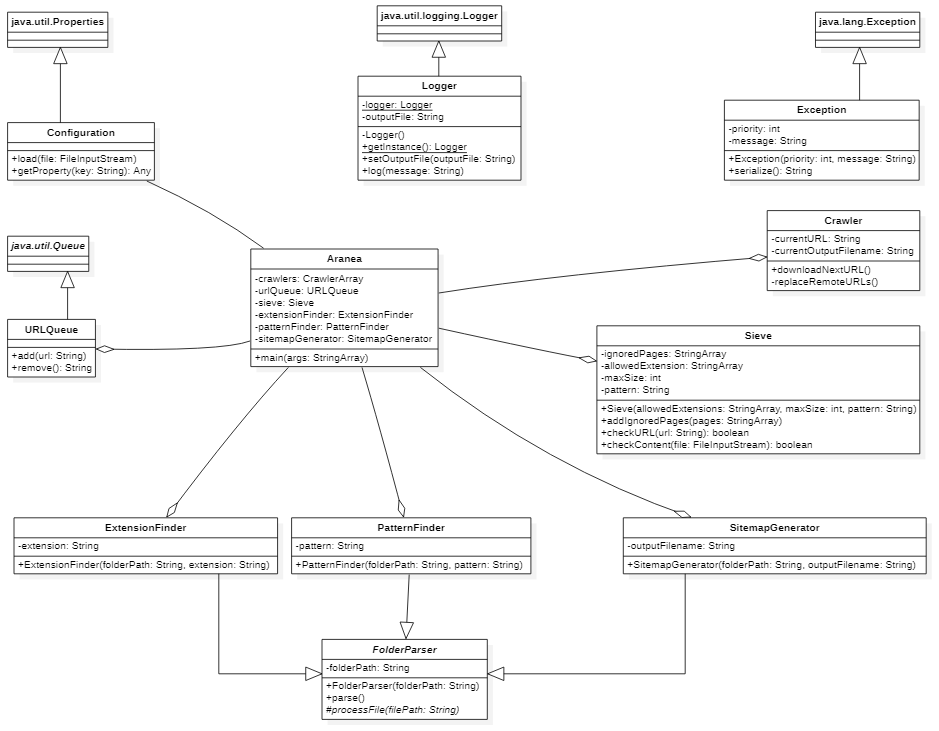
\includegraphics[width=15cm]{Class Diagram.png}
    \captionof{figure}{Diagramă de clase}
\end{center}

În diagramă, tipurile de date \mintinline{java}{DataArray} sunt o notație pentru \mintinline{java}{Data[]}. În plus, legăturile de asociere dintre anumite clase (\mintinline{java}{Configuration}, \mintinline{java}{Logger} și \mintinline{java}{Exception}), cât și clasele ce moștenesc \mintinline{java}{Exception}, au fost omise pentru a nu încărca diagrama. \\

\newpage

\subsection{Descriere a Claselor}

În tabelele următore, clasele \mintinline{java}{URLQueue} și \mintinline{java}{Configuration} au fost omise întrucât acestea au fost detaliate în cel cu \hyperlink{data_structures_link}{structuri de date globale}.

\begin{table}[H]
    \centering
    \begin{tabular}{ |p{0.25\linewidth} | p{0.75\linewidth}| } 
        \hline
        Nume & \mintinline{java}{Logger} \\
        Detalii despre Implementare & clasă Singleton, moștenire a clasei \href{https://docs.oracle.com/javase/7/docs/api/java/util/logging/Logger.html}{\mintinline{java}{java.util.loggin.Logger}} \\
        Descriere & Jurnalizează într-un fișier evenimentele întâmplate de-a lungul execuției. Poate fi folosită de către orice altă componentă pentru a avea acces la funcționalitatea de jurnalizare. \\
        Acțiuni Posibile & \begin{enumerate}
                               \item Preluarea instanței globale prin metoda \mintinline{java}{getInstance}
                               \item Setarea unui fișier de jurnalizare prin metoda \mintinline{java}{setOutputFile}
                               \item Jurnalizarea unui eveniment prin metoda \mintinline{java}{log}
                           \end{enumerate} \\
        \hline
    \end{tabular}
    \caption{Descriere a clasei \mintinline{java}{Logger}}
    \label{table:1}
\end{table}

\newpage

\begin{table}[H]
    \centering
    \begin{tabular}{ |p{0.25\linewidth} | p{0.75\linewidth}| } 
        \hline
        Nume & \mintinline{java}{Exception} \\
        Detalii despre Implementare & moștenire a clasei \href{https://docs.oracle.com/javase/7/docs/api/java/lang/Exception.html}{\mintinline{java}{java.lang.Exception}} \\
        Descriere & Reprezintă o excepție, putând fi moștenită în diferite alte clase ce descriu tipuri particulare de excepții. \\
        Acțiuni Posibile & \begin{enumerate}
                               \item Instanțierea și setarea priorității și a mesajului, prin intermediul constructorului
                               \item Serializarea informațiilor prin metoda \mintinline{java}{serialize}, ce presupune crearea unui șir de caractere cu formatul \mintinline{java}{"TIP_EVENIMENT: MESAJ"}, unde:
                                   \begin{itemize}
                                       \item \mintinline{java}{TIP_EVENIMENT} este \mintinline{java}{"INFO"} dacă prioritatea setată este 0, \mintinline{java}{"WARNING"} dacă prioritatea este 1, \mintinline{java}{"ERROR"} dacă prioritatea este 2 și \mintinline{java}{"CRITICAL"} dacă prioritatea este 3
                                       \item \mintinline{java}{MESAJ} este mesajul specific excepției.
                                   \end{itemize}
                           \end{enumerate} \\
    
        \hline
    \end{tabular}
    \caption{Descriere a clasei \mintinline{java}{Exception}}
    \label{table:1}
\end{table}

\newpage

\begin{table}[H]
    \centering
    \begin{tabular}{ |p{0.25\linewidth} | p{0.75\linewidth}| } 
        \hline
        Nume & \mintinline{java}{FolderParser} \\
        Detalii despre Implementare & clasă abstractă \\
        Descriere & Parcurge recursiv un director și efectuează o anumită operațiune pe baza fiecărui fișier găsit. \\
        Acțiuni Posibile & \begin{enumerate}
                               \item Instanțierea și setarea directorului prin intermediul constructorului
                               \item Începerea procesării prin metoda \mintinline{java}{parse}
                               \item Procesarea apelată la găsirea unui fișier, prin metoda virtuală \mintinline{java}{processFile}
                           \end{enumerate} \\
        \hline
    \end{tabular}
    \caption{Descriere a clasei \mintinline{java}{FolderParser}}
    \label{table:1}
\end{table}

\newpage

\begin{table}[H]
    \centering
    \begin{tabular}{ |p{0.25\linewidth} | p{0.75\linewidth}| } 
        \hline
        Nume & \mintinline{java}{ExtensionFinder} \\
        Detalii despre Implementare & implementare (prin moștenire) a clasei abstracte \mintinline{java}{FolderParser} \\
        Descriere & Parcurge recursiv un director și printează pe ecran numele fișierelor având o anumită extensie. \\
        Acțiuni Posibile & \begin{enumerate}
                               \item Instanțierea și setarea directorului și a extensiei prin intermediul constructorului
                           \end{enumerate} \\
        \hline
    \end{tabular}
    \caption{Descriere a clasei \mintinline{java}{ExtensionFinder}}
    \label{table:1}
\end{table}

\newpage

\begin{table}[H]
    \centering
    \begin{tabular}{ |p{0.25\linewidth} | p{0.75\linewidth}| } 
        \hline
        Nume & \mintinline{java}{PatternFinder} \\
        Detalii despre Implementare & implementare (prin moștenire) a clasei abstracte \mintinline{java}{FolderParser} \\
        Descriere & Parcurge recursiv un director și printează pe ecran numele fișierelor având conținut ce potrivește un anumit șablon. \\
        Acțiuni Posibile & \begin{enumerate}
                               \item Instanțierea și setarea directorului și a șablonului prin intermediul constructorului
                           \end{enumerate} \\
        \hline
    \end{tabular}
    \caption{Descriere a clasei \mintinline{java}{PatternFinder}}
    \label{table:1}
\end{table}

\newpage

\begin{table}[H]
    \centering
    \begin{tabular}{ |p{0.25\linewidth} | p{0.75\linewidth}| } 
        \hline
        Nume & \mintinline{java}{SitemapGenerator} \\
        Detalii despre Implementare & implementare (prin moștenire) a clasei abstracte \mintinline{java}{FolderParser} \\
        Descriere & Parcurge recursiv un director și creează o hartă, pe care o scrie, la finalizarea operației, într-un fișier. \\
        Acțiuni Posibile & \begin{enumerate}
                               \item Instanțierea și setarea directorului și a fișierului de ieșire prin intermediul constructorului
                           \end{enumerate} \\
        \hline
    \end{tabular}
    \caption{Descriere a clasei \mintinline{java}{SitemapGenerator}}
    \label{table:1}
\end{table}

\newpage

\begin{table}[H]
    \centering
    \begin{tabular}{ |p{0.25\linewidth} | p{0.75\linewidth}| } 
        \hline
        Nume & \mintinline{java}{Sieve} \\
        Detalii despre Implementare & \varnothing \\
        Descriere & Dă permisiunea ca un fișier să fie descărcat sau salvat local, pe baza unor criterii. Pe baza URL-ului, verifică dacă fișierul se află în \mintinline{bash}{robots.txt}, extensia și dimensiunea (printr-o cerere de tip \mintinline{bash}{HEAD}). În plus, poate verifica dacă un anumit șablon este potrivit de conținutul fișierului.\\
        Acțiuni Posibile & \begin{enumerate}
                               \item Instanțierea și setarea extensiilor permise, a dimensiunii maxime și a unui șablon prin intermediul constructorului
                               \item Adăugarea unor fișiere ce se află în \mintinline{bash}{robots.txt}, prin metoda \mintinline{java}{addIgnoredPages}
                               \item Verificarea unui URL prin metoda \mintinline{java}{checkURL}
                               \item Verificarea conținutului unui fișier prin metoda \mintinline{java}{checkContent}
                           \end{enumerate} \\
        \hline
    \end{tabular}
    \caption{Descriere a clasei \mintinline{java}{Sieve}}
    \label{table:1}
\end{table}

\newpage

\begin{table}[H]
    \centering
    \begin{tabular}{ |p{0.25\linewidth} | p{0.75\linewidth}| } 
        \hline
        Nume & \mintinline{java}{Crawler} \\
        Detalii despre Implementare & clasă tip worker (fiecare instanță rulează pe un fir de execuție separat) \\
        Descriere & Descarcă pagini salvate în coada de tip \mintinline{java}{URLQueue}. După salvarea lor, parcurge conținutul fișierului și înlocuiește toate URL-urile externe întâlnite cu unele către fișierel locale.  De specificat este faptul că toate cererile vor fi efectuate cu un agent specific, \mintinline{java}{AraneaBot}.\\
        Acțiuni Posibile & \begin{enumerate}
                               \item Descărcarea unei pagini prin metoda \mintinline{java}{downloadNextURL}
                               \item Înlocuirea URL-urilor din fișierele savate prin metoda privată \mintinline{java}{replaceRemoteURLs}
                           \end{enumerate} \\
        \hline
    \end{tabular}
    \caption{Descriere a clasei \mintinline{java}{Crawler}}
    \label{table:1}
\end{table}

\newpage

\begin{table}[H]
    \centering
    \begin{tabular}{ |p{0.25\linewidth} | p{0.75\linewidth}| } 
        \hline
        Nume & \mintinline{java}{Aranea} \\
        Detalii despre Implementare & \varnothing \\
        Descriere & Este inițializată la apelarea metodei \mintinline{java}{main}, pe baza parametrilor programului. Cuprinde majoritatea celorlaltor clase descrise, orchestrându-le astfel încât execuția să fie de succes: 
            \begin{itemize}
                \item pentru operațiunea de crawling
                \begin{itemize}
                    \item inițializează configurația de tip \mintinline{java}{Configuration}, pe baza fișierului de configurare
                    \item inițializează coada de pagini, de tip \mintinline{java}{URLQueue}, pe baza fișierului de intrare și a fișierelor \mintinline{bash}{robots.txt} specifice lor
                    \item inițializează un filtru pentru paginile descărcate, prin intermediul clasei \mintinline{java}{Sieve}
                    \item creează fire de execuție pentru fiecare instanță a clasei \mintinline{java}{Crawler}
                    \item dacă se dorește crearea de hărți, instanțiază un obiect de tipul \mintinline{java}{SitemapGenerator}
                \end{itemize}
                \item pentru operațiunea de căutare a fișierelor cu o anumită extensie, instanțiază un obiect de tipul \mintinline{java}{ExtensionFinder}
                \item pentru operațiunea de căutare a fișierelor cu conținut ce potrivește un anumit șablon, instanțiază un obiect de tipul \mintinline{java}{PatternFinder}
            \end{itemize} \\
        Acțiuni Posibile & \varnothing \\
        \hline
    \end{tabular}
    \caption{Descriere a clasei \mintinline{java}{Aranea}}
    \label{table:1}
\end{table}

\newpage

\section{Modelare a Interfeței cu Utilizatorul}

Interfațarea cu utilizatorul se realizează prin intermediul liniei de comandă. Cum programul este distribuit sub forma unei arhive JAR, acesta poate fi rulat cu ajutorul comenzii \mintinline{bash}{java -jar ABSOLUTE_PATH_TO/aranea.jar COMMAND [ARGUMENTS]}. Din cauza dificultății ei, o adăugare a unui alias va fi recomandată utilizatorilor, cu ajutorul uneia dintre comenzile următoare:
\begin{itemize}
    \item \mintinline{bash}{doskey aranea=java -jar ABSOLUTE_PATH_TO/aranea.jar} pentru sistemele de operare Windows
    \item \mintinline{bash}{alias aranea=java -jar ABSOLUTE_PATH_TO/aranea.jar} pentru sistemele de operare Linux și macOS.
\end{itemize} \\
Utilizatorii vor putea rula următoarele comenzi pentru a folosi Aranea:
\begin{itemize}
    \item \mintinline{bash}{aranea crawl URLS_FILE CONFIG_FILE} pentru executarea crawling-ului pe o serie de website-uri
    \item \mintinline{bash}{aranea crawl list EXTENSION} pentru listarea fișierelor salvate local, cu o anumită extensie
    \item \mintinline{bash}{aranea crawl search PATTERN} pentru căutarea unui șablon în paginile salvate local
    \item \mintinline{bash}{aranea} sau \mintinline{bash}{aranea help} pentru soliciarea ajutorului.
\end{itemize} \\
În funcție de operațiune, utilizatorilor li se poate afișa text pe ecran sau oferi fișiere locale pe care să le verifice manual, ulterior.

\newpage

\section{Elemente de Testare}

Testarea aplicației rezultate în urma perioadei de implementare va fi realizată conform cu următoarea metodologie:
\begin{enumerate}
    \item Crearea a două teste automate (unul cu dificultate scăzută și unul cu dificultate ridicată) pentru fiecare caz de utilizare, cu ajutorul JUnit
    \item Rularea testelor și observarea rezultatelor
    \item Consemnarea funcționării incorecte a aplicației în secțiunea de probleme a Github și rezolvarea individuală sau colaborativă a problemei.
\end{enumerate}

\end{document}